\documentclass{article}

\usepackage{amsmath,amssymb}
\usepackage{tikz}
\usepackage{pgfplots}
\usepackage{xcolor}
\usepackage[left=2.1cm,right=3.1cm,bottom=3cm,footskip=0.75cm,headsep=0.5cm]{geometry}
\usepackage{enumerate}
\usepackage{enumitem}
\usepackage{marvosym}
\usepackage{tabularx}
\usepackage{parskip}

\usepackage{listings}
\lstdefinelanguage{JavaScript}{
	keywords={typeof, new, true, false, catch, function, return, null, catch, switch, var, if, in, while, do, else, case, break, for, of, document},
	keywordstyle=\color{lila}\bfseries,
	ndkeywords={class, export, boolean, throw, implements, import, this},
	ndkeywordstyle=\color{lila}\bfseries,
	identifierstyle=\color{blue},
	sensitive=false,
	comment=[l]{//},
	morecomment=[s]{/*}{*/},
	commentstyle=\color{lightgray}\ttfamily,
	stringstyle=\color{mygreen}\ttfamily,
	morestring=[b]',
	morestring=[b]"
}
\definecolor{lightlightgray}{rgb}{0.95,0.95,0.95}
\definecolor{lila}{rgb}{0.8,0,0.8}
\definecolor{mygray}{rgb}{0.5,0.5,0.5}
\definecolor{mygreen}{rgb}{0,0.8,0.26}
\lstdefinestyle{xml} {language=xml, morekeywords={encoding, newspaper, article, title, id, published, author, xs:schema, xmlns:xs, xs:element, name, xs:sequence, xs:element, type, xs:complexType}}
\lstdefinestyle{json}{}
\lstdefinestyle{javascript}{language=javascript}
\lstdefinestyle{html}{language=html, morekeywords={main}}
\lstset{language=XML,
	basicstyle=\ttfamily,
	keywordstyle=\color{lila},
	commentstyle=\color{lightgray},
	stringstyle=\color{mygreen}\ttfamily,
	backgroundcolor=\color{white},
	showstringspaces=false,
	numbers=left,
	numbersep=10pt,
	tabsize=2,
	numberstyle=\color{mygray}\ttfamily,
	identifierstyle=\color{blue},
	xleftmargin=.1\textwidth, 
	%xrightmargin=.1\textwidth,
	escapechar=§,
	%literate={\t}{{\ }}1
	breaklines=true,
	postbreak=\mbox{\space},
	literate=%
	{Ö}{{\"O}}1
	{Ä}{{\"A}}1
	{Ü}{{\"U}}1
	{ß}{{\ss}}1
	{ü}{{\"u}}1
	{ä}{{\"a}}1
	{ö}{{\"o}}1
}

\usepackage[colorlinks = true, linkcolor = blue, urlcolor  = blue, citecolor = blue, anchorcolor = blue]{hyperref}
\usepackage[utf8]{inputenc}

\renewcommand*{\arraystretch}{1.4}

\newcolumntype{L}[1]{>{\raggedright\arraybackslash}p{#1}}
\newcolumntype{R}[1]{>{\raggedleft\arraybackslash}p{#1}}
\newcolumntype{C}[1]{>{\centering\let\newline\\\arraybackslash\hspace{0pt}}m{#1}}

\newcommand{\E}{\mathbb{E}}
\DeclareMathOperator{\rk}{rk}
\DeclareMathOperator{\Var}{Var}
\DeclareMathOperator{\Cov}{Cov}

\title{\textbf{Internet and Web Applications, Übung 2}}
\author{\textsc{Henry Haustein}}
\date{}

\begin{document}
	\maketitle
	
	\section*{Aufgabe 1: Representational State Transfer}
	Die Vorteile sind
	\begin{itemize}
		\item Skalierbarkeit: Client und Server sind getrennt
		\item Flexibilität: API kann ohne Probleme von einem Server zu einem Server portiert werden
		\item Unabhängigkeit: REST ist unabhängig von der restlichen Architektur
	\end{itemize}

	\section*{Aufgabe 2: TCP Fast Open}
	TCP Fast Open wurde entwickelt um Daten direkt beim Handshake mit auszutauschen. Damit spart man sich eine voll Round-Trip-Time bevor Daten ausgetauscht werden können (beim klassischen TCP). Man steigert die Effizienz.
	
	Aus \url{https://datatracker.ietf.org/doc/html/rfc7413}: Performing TCP Fast Open:
	\begin{enumerate}[label=\arabic*.]
		\item The client sends a SYN with data and the cookie in the Fast Open option.
		\item The server validates the cookie:
		\begin{itemize}
			\item If the cookie is valid, the server sends a SYN-ACK acknowledging both the SYN and the data.  The server then delivers the data to the application.
			\item Otherwise, the server drops the data and sends a SYN-ACK acknowledging only the SYN sequence number.
		\end{itemize}
		\item If the server accepts the data in the SYN packet, it may send the response data before the handshake finishes.  The maximum amount is governed by TCP's congestion control [RFC5681].
		\item The client sends an ACK acknowledging the SYN and the server data. If the client's data is not acknowledged, the client retransmits the data in the ACK packet.
		\item The rest of the connection proceeds like a normal TCP connection. The client can repeat many Fast Open operations once it acquires a cookie (until the cookie is expired by the server).  Thus, TFO is useful for applications that have temporal locality on client and server connections.
	\end{enumerate}
	\begin{center}
		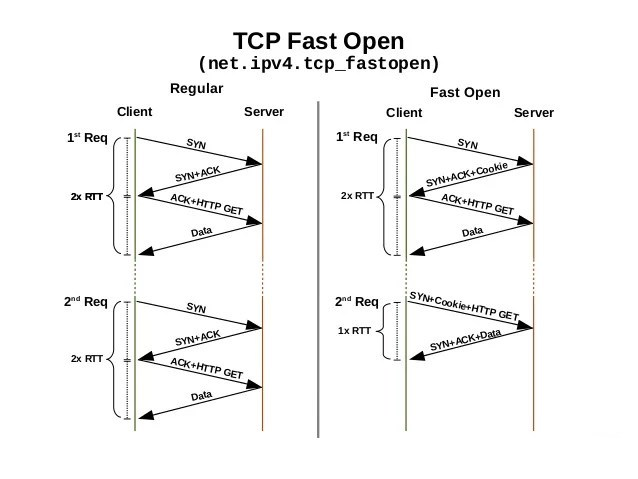
\includegraphics[scale=0.6]{tcp_fast_open}
	\end{center}
	
	\section*{Aufgabe 3: HTTP/2 and HTTP/3}
	\begin{enumerate}[label=(\alph*)]
		\item HTTP/2 stellt einen schnelleren Transport der Daten durch Multiplexing und Header-Komprimierung sicher. In einer TCP Verbindung können mehrere Channel aufgebaut werden und damit mehrere Requests parallel verarbeitet werden. \\
		Aus \url{https://datatracker.ietf.org/doc/html/draft-ietf-quic-http-27}: \textit{HTTP/2 introduced a binary framing and multiplexing layer to improve latency without modifying the transport layer.  However, because the parallel nature of HTTP/2's multiplexing is not visible to TCP's loss recovery mechanisms, a lost or reordered packet causes all active transactions to experience a stall regardless of whether that transaction was impacted by the lost packet.}
		\item  Unterschiede:
		\begin{itemize}
			\item HTTP/3 basiert auf QUIC und nicht mehr auf TCP
			\item TLS 1.3 auf QUIC-Ebene
			\item konstante Verbindung $\to$ weniger Datenpakete, weil kein Header jedes mal gesendet werden muss
			\item Fehlerkorrektur auf QUIC-Ebene
			\item bei Paketverlusten stockt die Verbindung nicht mehr, weil nicht mehr gewartet werden muss
			\item HTTP/3 verzichtet auf einleitende Handshakes
			\item HTTP/3 ist nicht mehr an IP-Adressen gebunden, sondern an individuelle Verbindungs-IDs, die selbst bei einem Netzwerkwechsel einen konstanten Download ermöglichen
		\end{itemize}
	\end{enumerate}
	
	\section*{Aufgabe 4: Cookie mechanism}
	\begin{enumerate}[label=(\alph*)]
		\item Cookies sind Key-Value-Paare, die bei jedem Requests vom Browser im Header-Feld \texttt{cookie} mitgesendet werden. Der Server kann in der Response auch Cookies mittels Header-Feld \texttt{set-cookie} setzen.
		\item mittels Header-Feld \texttt{authentication: bearer <token>}, mittels PHP-Session-IDs, mittels Fingerprinting (\url{https://amiunique.org/fp})
	\end{enumerate}

\end{document}